\documentclass[12pt,a4paper]{article}
\usepackage[left=2cm,right=2cm,top=2cm,bottom=2cm]{geometry}
\usepackage{amsfonts}
\usepackage{amsmath}
\usepackage{enumitem}
\usepackage{tikz}
\usepackage{pgfplots}

\usetikzlibrary{calc,matrix,backgrounds}

\pgfdeclarelayer{overlay}
\pgfsetlayers{overlay,background,main}

\tikzset{circle/.style = {rounded corners,line width=1bp,color=#1}}%

\newcommand{\pvec}[2]{\begin{pmatrix} #1 \\ #2\end{pmatrix}}
\newcommand{\reals}{\mathbb{R}}
\newcommand{\drawgraph}{\draw[-] (-1, 0) -- (1, 0) node[right] {$x$};
\draw[-] (0, -1) -- (0, 1) node[above] {$y$};}

\title{Funcions}
\author{-}
\date{Febrer 2023}

\pgfplotsset{compat=1.18}
\begin{document}

\maketitle

\section{Models Funcionals}

\subsection{Polinòmiques}
\subsubsection{Cosntant}

\begin{minipage}[t]{0.4\textwidth}
    \begin{align*}
        \begin{tikzpicture}
            \begin{axis}[
                domain=-5:5,
                samples=100,
                width=150pt,
                height=150pt,
                axis lines=middle,
                enlarge x limits=false,
                no markers,
                axis equal,
                legend pos = outer north east,
                xlabel={$x$},
                ylabel={$y$}]
                \addplot[blue, domain=-5:5] {2};
                \legend{$2$}
                \end{axis}
        \end{tikzpicture}
    \end{align*}
\end{minipage}
\begin{minipage}[t]{0.5\textwidth}
    \begin{enumerate}[label=-]
        \item $f(x) = k$
        \item La imatge és igual a tota la funció $\rightarrow Im(f) = k$
        \item És una recta horiztonal
        \item El domini són tots els $\reals$ $\rightarrow$ $Dom(f) = \reals$
    \end{enumerate}
\end{minipage}

\subsubsection{Afí o lineal}
\begin{minipage}[t]{0.4\textwidth}
    \begin{align*}
        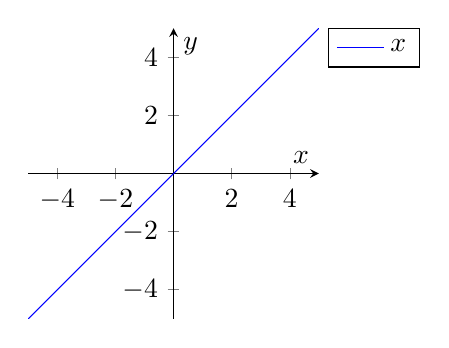
\begin{tikzpicture}
            \begin{axis}[
                domain=-5:5,
                samples=100,
                width=150pt,
                height=150pt,
                axis lines=middle,
                enlarge x limits=false,
                no markers,
                legend pos = outer north east,
                xlabel={$x$},
                ylabel={$y$}]
              \addplot[blue, domain=-5:5] {x};
              \legend{$x$}
              \end{axis}
        \end{tikzpicture}
    \end{align*}
\end{minipage}
\begin{minipage}[t]{0.5 \textwidth}
    \begin{enumerate}[label=-]
        \item $f(x)=mx+n$
        \item Polinomi de 1r grau
        \item $m$ = pendent
        \item $Dom(f)=\reals$
        \item $Im(f)=\reals$
    \end{enumerate}
\end{minipage}
\subsubsection{Quadràtica}
\begin{minipage}[t]{0.4\textwidth}
    \begin{align*}
        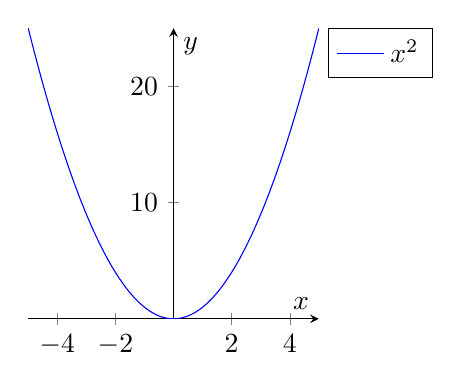
\begin{tikzpicture}
            \begin{axis}[
                domain=-5:5,
                samples=100,
                width=150pt,
                height=150pt,
                axis lines=middle,
                enlarge x limits=false,
                no markers,
                legend pos = outer north east,
                xlabel={$x$},
                ylabel={$y$}]
              \addplot[blue, domain=-5:5] {x^2};
              \legend{$x^2$}
              \end{axis}
        \end{tikzpicture}
    \end{align*}
\end{minipage}
\begin{minipage}[t]{0.5\textwidth}
    \begin{enumerate}[label=-]
        \item $f(x)=ax^2+bx+c$
        \item Polinomi de 2n grau
        \item $Dom(f)= \reals$
        \item És una parabola
    \end{enumerate}
\end{minipage}
\subsubsection{Polinòmiques}
\begin{enumerate}[label=-]
    \item \underline{Grau Senar}\\
        \begin{minipage}[t]{0.4\textwidth}
            \begin{align*}
                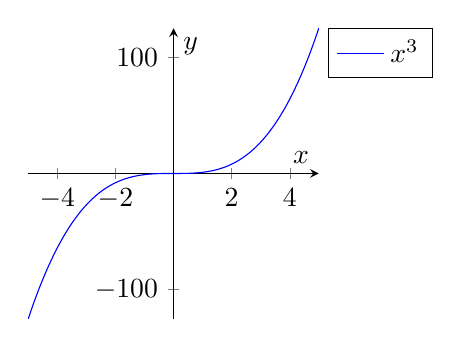
\begin{tikzpicture}
                    \begin{axis}[
                        domain=-5:5,
                        samples=100,
                        width=150pt,
                        height=150pt,
                        axis lines=middle,
                        enlarge x limits=false,
                        no markers,
                        legend pos = outer north east,
                        xlabel={$x$},
                        ylabel={$y$}]
                      \addplot[blue, domain=-5:5] {x^3};
                      \legend{$x^3$}
                      \end{axis}
                \end{tikzpicture}
            \end{align*}
        \end{minipage}
        \begin{minipage}[t]{0.5\textwidth}
            \begin{enumerate}[label=-]
                \item $f(x)=ax^3+bx^2+cx+d$
                \item $Dom(f)=\reals$
                \item $Im(f)=\reals$
            \end{enumerate}
        \end{minipage}
    \item \underline{Grau parell}\\
    \begin{minipage}[t]{0.4\textwidth}
        \begin{align*}
            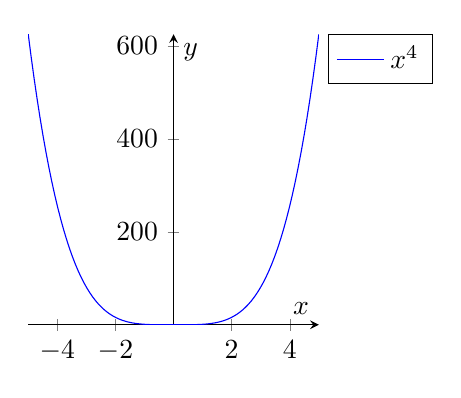
\begin{tikzpicture}
                \begin{axis}[
                    domain=-5:5,
                    samples=100,
                    width=150pt,
                    height=150pt,
                    axis lines=middle,
                    enlarge x limits=false,
                    no markers,
                    legend pos = outer north east,
                    xlabel={$x$},
                    ylabel={$y$}]
                  \addplot[blue, domain=-5:5] {x^4};
                  \legend{$x^4$}
                  \end{axis}
            \end{tikzpicture}
        \end{align*}
    \end{minipage}
    \begin{minipage}[t]{0.5\textwidth}
        \begin{enumerate}[label=-]
            \item $f(x)=ax^4+bx^3+cx^2+dx+k$
            \item $Dom(f)=\reals$
            \item $Im(f)\neq\reals$
        \end{enumerate}
    \end{minipage}
\end{enumerate}

\subsection{Racionals}
\begin{minipage}[t]{0.35\textwidth}
    \begin{align*}
        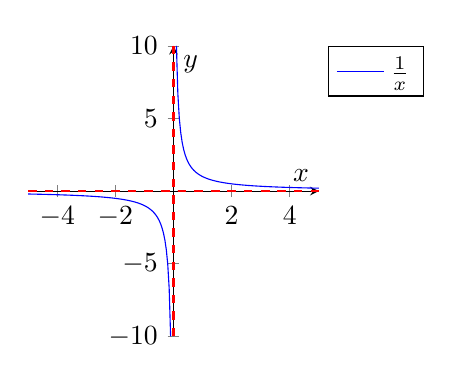
\begin{tikzpicture}
            \begin{axis}[
                domain=-5:5,
                samples=100,
                width=150pt,
                height=150pt,
                axis lines=middle,
                enlarge x limits=false,
                no markers,
                legend pos = outer north east,
                xlabel={$x$},
                ylabel={$y$}]
              \addplot[blue, domain=-5:-0.1] {1/x};
              \addplot[blue, domain=0.1:5] {1/x};
              \addplot[red, thick, dashed, domain=-5:5] {0};
              \addplot[red, thick, dashed] coordinates {(0, -10) (0, 10)};
              \legend{$\frac{1}{x}$}
              \end{axis}
        \end{tikzpicture}
    \end{align*}        
\end{minipage}
\begin{minipage}[t]{0.6\textwidth}
    \begin{enumerate}[label=-]
        \item $f(x)=\dfrac{1}{x}$
        \item $Dom(f)=\{x\in\reals / denominador \neq 0\}$
        \item Asintotes verticals i horitzontals o obliqües
    \end{enumerate}
\end{minipage}

\subsection{Irracionals}
\subsubsection{Senars}
\begin{minipage}[t]{0.4\textwidth}
    \begin{align*}
        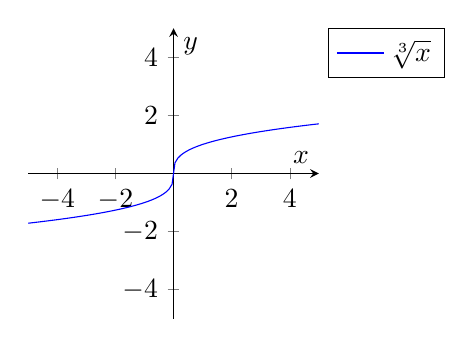
\begin{tikzpicture}
            \begin{axis}[
                domain=-5:5,
                samples=100,
                width=150pt,
                height=150pt,
                axis lines=middle,
                enlarge x limits=false,
                no markers,
                axis equal,
                legend pos = outer north east,
                xlabel={$x$},
                ylabel={$y$}]
              \addplot[blue] {x/abs(x)*abs(x)^(1/3)};
              \legend{$\sqrt[3]{x}$}
              \end{axis}
        \end{tikzpicture}
    \end{align*}
\end{minipage}
\begin{minipage}[t]{0.5\textwidth}
    \begin{enumerate}[label=-]
        \item $f(x)=\sqrt[n]{x}$, n és imparell
        \item $Dom(f)=\reals$
        \item $Im(f)=\reals$
    \end{enumerate}
\end{minipage}
\subsubsection{Parell}
\begin{minipage}[t]{0.4\textwidth}
    \begin{align*}
        \begin{tikzpicture}
            \begin{axis}[
                domain=0:10,
                samples=100,
                width=150pt,
                height=150pt,
                axis lines=middle,
                enlarge x limits=false,
                no markers,
                legend pos = outer north east,
                xlabel={$x$},
                ylabel={$y$}]
              \addplot[blue] {sqrt(x)};
              \legend{$\sqrt{x}$}
              \end{axis}
        \end{tikzpicture}
    \end{align*}
\end{minipage}
\begin{minipage}[t]{0.5\textwidth}
    \begin{enumerate}[label=-]
        \item $f(x)=\sqrt[n]{x}$, n és parell
        \item $Dom(f)=\{x\in\reals / radicant \geq 0\}$
    \end{enumerate}
\end{minipage}
\subsection{Exponencial}
\begin{minipage}[t]{0.4\textwidth}
    \begin{align*}
        \begin{tikzpicture}
            \begin{axis}[
                domain=-5:5,
                samples=100,
                width=150pt,
                height=150pt,
                axis lines=middle,
                enlarge x limits=false,
                no markers,
                legend pos = outer north east,
                xlabel={$x$},
                ylabel={$y$}]
              \addplot[blue] {e^x};
              \addplot[red, thick, dashed] {0};
              \legend{$e^x$}
              \end{axis}
        \end{tikzpicture}
    \end{align*}
\end{minipage}
\begin{minipage}[t]{0.5\textwidth}
    \begin{enumerate}[label=-]
        \item $f(x)=a^x$, $a > 0$
        \item $Dom(f)=\reals$
        \item Té una asintota horitzontal
    \end{enumerate}
\end{minipage}
\subsection{Logarítmiques}
\begin{minipage}[t]{0.4\textwidth}
    \begin{align*}
        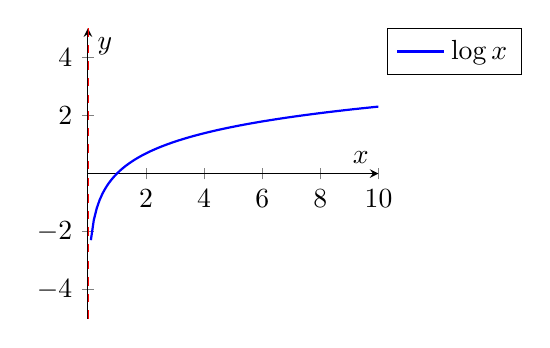
\begin{tikzpicture}
            \begin{axis}[
                domain=0:10,
                samples=100,
                width=150pt,
                height=150pt,
                axis lines=middle,
                enlarge x limits=false,
                no markers,
                axis equal,
                legend pos = outer north east,
                xlabel={$x$},
                ylabel={$y$}]
              \addplot +[thick] {ln(x)};
              \addplot[red, thick, dashed] coordinates {(0, -5) (0, 5)};
              \legend{$\log{x}$}
              \end{axis}        
        \end{tikzpicture}
    \end{align*}
\end{minipage}
\begin{minipage}[t]{0.5\textwidth}
    \begin{enumerate}[label=-]
        \item $f(x)=\log{(x)}$
        \item $Dom(f)=\{x\in\reals / "lo de dintre" > 0\}$
        \item $Im(f)=\reals$
        \item Té uina asintota vertical
    \end{enumerate}
\end{minipage}
\subsection{Trigonometriques}
\subsubsection{Cosinus i Sinus}
\begin{minipage}[t]{0.4\textwidth}
    \begin{align*}
        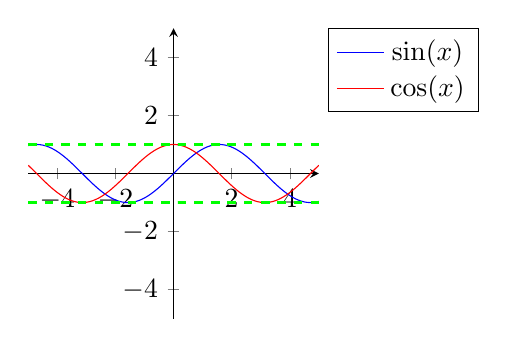
\begin{tikzpicture}
            \begin{axis}[
                domain=-5:5,
                samples=100,
                width=150pt,
                height=150pt,
                axis lines=middle,
                enlarge x limits=false,
                no markers,
                axis equal,
                legend pos = outer north east
            ]
             \addplot {sin(deg(x))};
             \addplot {cos(deg(x))};
             \addplot[green, thick, dashed] {1};
             \addplot[green, thick, dashed] {-1};
             \legend{$\sin(x)$, $\cos(x)$}
            \end{axis}
        \end{tikzpicture}
    \end{align*}
\end{minipage}
\begin{minipage}[t]{0.5\textwidth}
    \begin{enumerate}[label=-]
        \item $f(x)=\sin(x)$
        \item $g(x)=\cos(x)$
        \item Periodiques
        \item $Dom(f, g)=\reals$
        \item Acotades (cota superior i cota inferior)
    \end{enumerate}
\end{minipage}
\subsubsection{tangent}
\begin{minipage}[t]{0.4\textwidth}
    \begin{align*}
        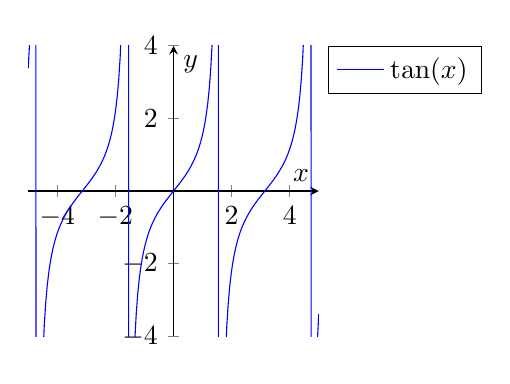
\begin{tikzpicture}
            \begin{axis}[
                domain=-5:5,
                ymin=-4, ymax=4,
                samples=100,
                width=150pt,
                height=150pt,
                axis lines=middle,
                enlarge x limits=false,
                no markers,
                legend pos = outer north east,
                xlabel={$x$},
                ylabel={$y$}
                ]
              \addplot[blue,samples=200] {tan(deg(x))}node[right]{$y=\tan x$};
            \legend{$\tan(x)$}
            \end{axis}
        \end{tikzpicture}
    \end{align*}
\end{minipage}
\begin{minipage}[t]{0.5\textwidth}
    \begin{enumerate}[label=-]
        \item $f(x)=\tan(x)$
        \item $Dom(f)=\{x\in\reals / l'angle \neq \frac{\pi}{2}+\pi\cdot k\}$
        \item Periodica
        \item $Im(f)=\reals$
        \item Té $\infty$ AV
    \end{enumerate}
\end{minipage}

\section{Concepte de funció}
Una funció nomes pot torbar un valor def la variable dependent ($y$) per un valor de la variable independent ($x$).\\
Si la funcio $f(4) = (2, 7)$ la funció $f$ no és una funció.\\
Si $x_1\neq x_2 \Longrightarrow f(x_1) \neq f(x_2)$, llavors, $f$ és una funció injectiva, no hi han dos valors de $x$ que donguin el mateix resultat.\\
Per calcular la imatge d'una funció, $f(x), x\in Dom(f)$\\
Per calcular la antimage d'una funció, $f^{-1}(x)$

\subsection{Funcins a trossos}

\begin{align*}
    F(x)= \left\{ \begin{array}{lcc}
        f(x) & si & x < 0 \\
        g(x) & si & x \geq 0 
        \end{array}
    \right.
\end{align*}
Exemple:
\begin{align*}
    F(x) = \left\{ \begin{array}{lcc}
        x^2 & si & x\leq 0 \\
        \sin x & si & 0 < x < 2\\
        e^x-2 & si & x > 2
    \end{array}
    \right.
\end{align*}
$Dom(F)=\reals-\{2\}$
\section{Transformació de funcions}
\subsection{Translacions}
Desplaçamenty de tota la funció\\
Si $f(x)$ és la funció inicial
\begin{enumerate}[label=$\to$]
    \item Translació horitzontal: $y=f(x-a)$, desplaçament de a unitats, si $a>0$ desplaçament cap a la dreta, si $a<0$ desplaçament cap a l'esquerra.
    \item Translació vertical: $y=f(x)+b$, desplaçament de $b$ unitats, si $b>0$ desplaçament cap amunt, si $b<0$ desplaçament cap avall.
\end{enumerate}

\begin{align*}
    $y=f(x-a)+b$\text{, }$f$  \text{està traslladada amb el vector} $\pvec{a}{b}$
\end{align*}


\end{document}
